\documentclass{article}
\usepackage[utf8]{inputenc}
\usepackage{natbib}
\usepackage{graphicx}
\usepackage{fancyhdr}
\usepackage{float}
\usepackage{enumerate}
\pagestyle{fancy}
\usepackage{xcolor}
\usepackage{subcaption}
\definecolor{gold}{RGB}{255,215,0}
\definecolor{night-blue}{RGB}{26,72,118}
\definecolor{manatee}{RGB}{151,154,170}
\definecolor{purple}{RGB}{188,143,143}
\definecolor{yellow}{RGB}{255,211,92}
\definecolor{salmon}{RGB}{255,160,122}
\definecolor{verde}{RGB}{188,218,185}
 
\begin{document}

\begin{titlepage}

\newcommand{\HRule}{\rule{\linewidth}{0.5mm}} % Defines a new command for the horizontal lines, change thickness here

\center % Center everything on the page
 
 

\textsc{\large DIVISIÓN DE INGENIERÍAS CAMPUS IRAPUATO - SALAMANCA}\\[1.5cm] 

\includegraphics[scale=.8]{images/descarga.jpg}\\[1cm]  
\textsc{\Large Redes de computadoras I}\\[0.5cm]  
 

\HRule \\[.8cm]
\textbf{\bfseries Práctica 3}\\[0.4cm] % Title of your document
\HRule \\[1.5cm]
 
%----------------------------------------------------------------------------------------
%	AUTHOR SECTION
%----------------------------------------------------------------------------------------

 
\begin{center}
   \textcolor{night-blue}{Adán Hernández Baena : 146062\\}
\end{center}

\bigskip
    {\large \today}\\[2cm] % Date, change the \today to a set date if you want to be precise

\vfill % Fill the rest of the page with whitespace

\end{titlepage}

\newpage
\pagestyle{fancy}
\fancyhf{}
\rhead{Intermediate Practice}
\lhead{Data Mining}
\rfoot{ \thepage} 
%\tableofcontents
\newpage
\section{StackOverflow users' data}
The data consists of a bunch of some users' information from StackOverflow website. The data is stored on a csv file with \textbf{88883 rows} and \textbf{10 columns} where each row means a user's answers (the data were collected from a survey) and the columns indicate the questions. The columns headers are Country, Education Level, Developer type, Years of coding, Salary in USD, Worked hours per week, Languages that they have used, Age, Gender and Ethnicity.
After a superficial look to the csv, a realized that the answers are too homogeneous, then I was not going to need to do much data cleaning (as lowercase converting, remove excess of blanks values, etc) the "only problem" were the multiple answers and some dispersed null values.
As first step I considered the visualization of the data distribution of the salary according other variable (Education level, ).
\section{Salaries distribution}
Observing the salaries respect to developer type, gender, country, educational level, etc, (Figures~\ref{fig:salarybygenderhist} to~\ref{fig:salarybyethnicityhist}) do not influence much of the distributions of these, the salaries are concentrated around 40K and 50K USD per year. Therefore, any variable does not influence on salary distribution, you can starve of death or you could earn until 2 millions USD regardeless your education, age, gender, age, etc.
Another thing that made me interesting to analyze was whether the amount of programming language that someone has worked with influence in the salaries. The results are shown on Figure~\ref{fig:salarybylang1} to~\ref{fig:salarybylang}, where it could be observed how the more programming languages means in less programmers and the average increase a bit.
\begin{figure}[ht]
    \centering
    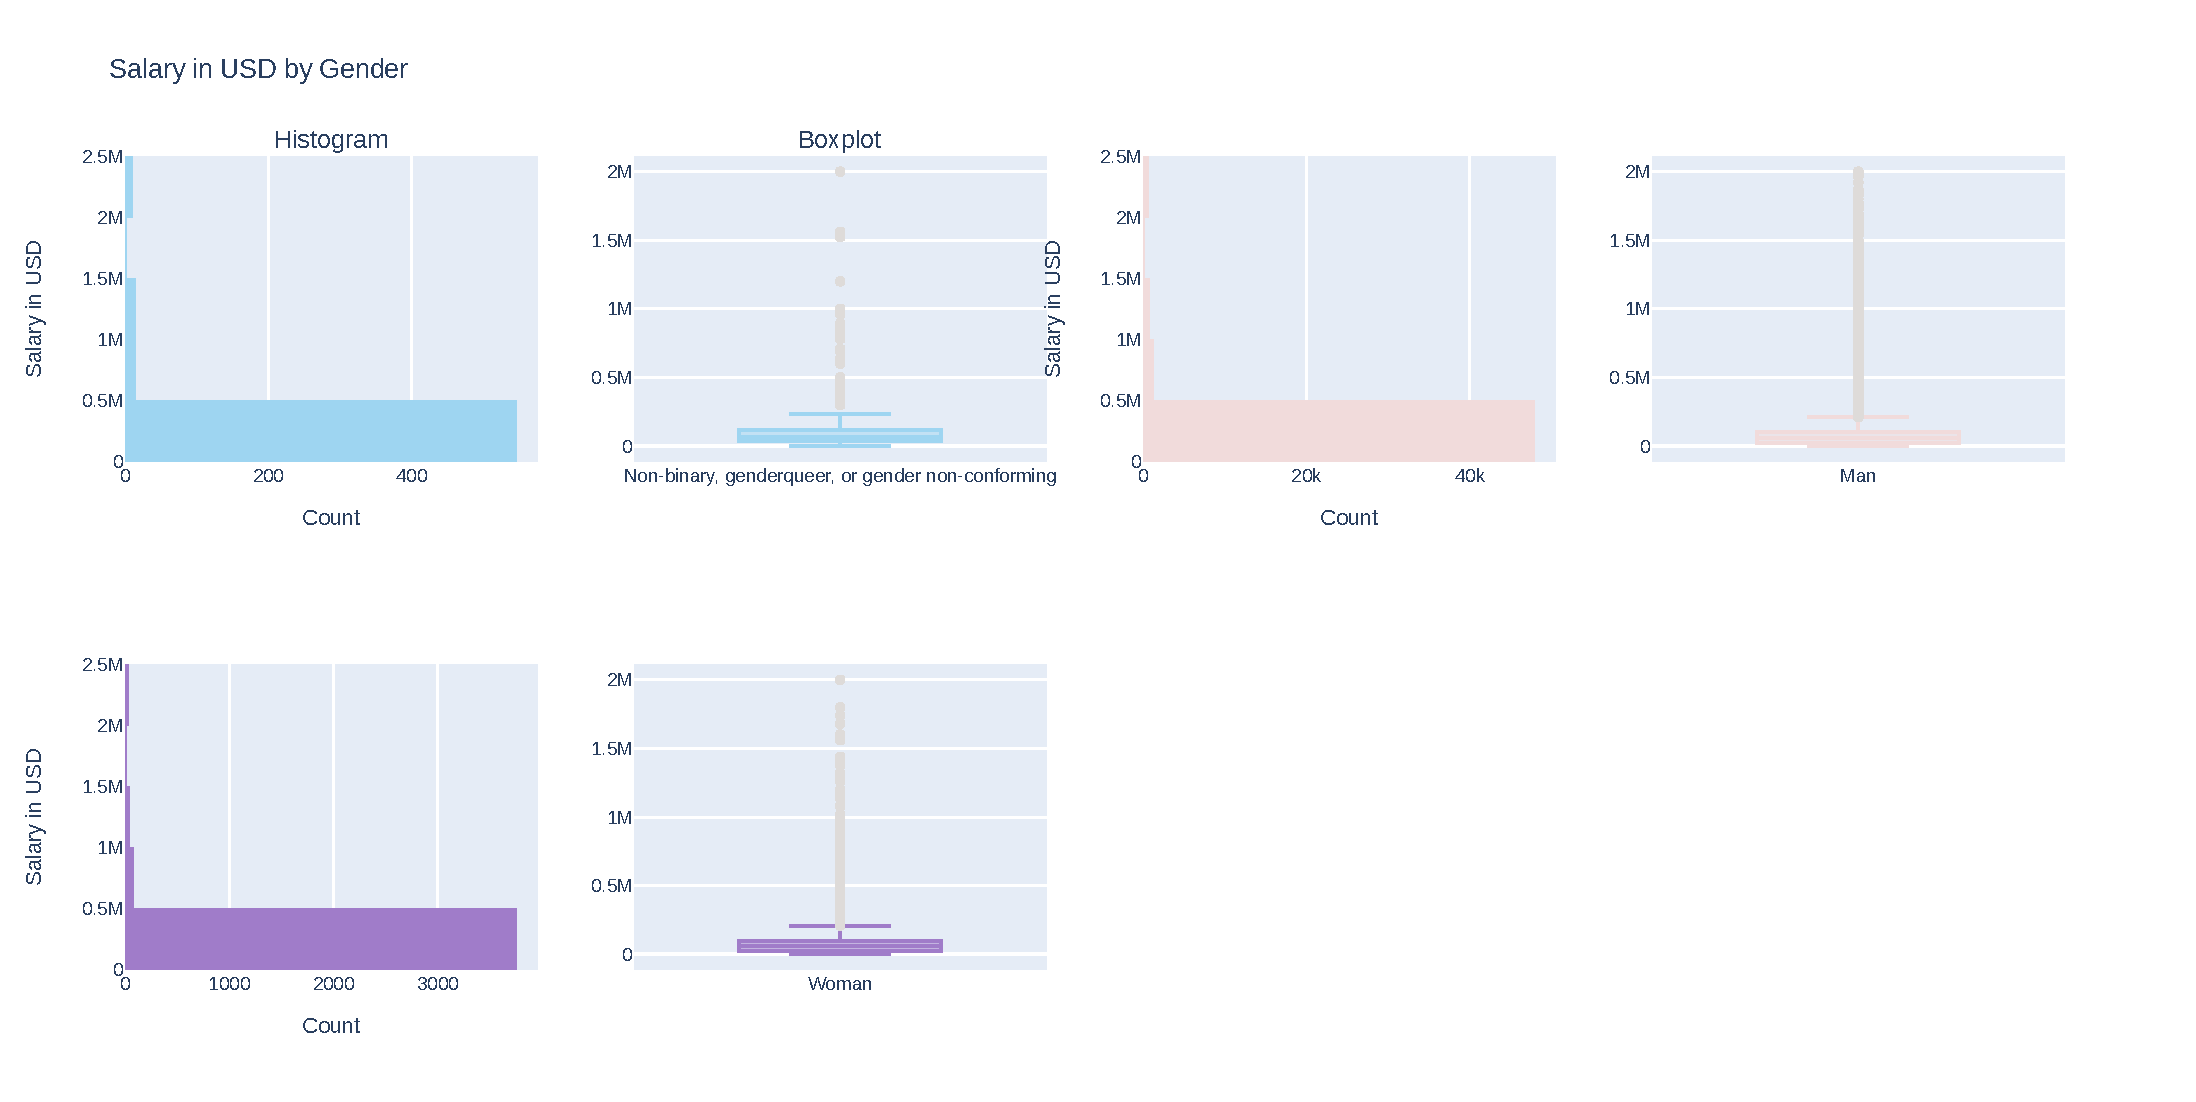
\includegraphics[width=\textwidth]{images/salary_gender_hist.pdf}
    \caption{Distribution of Salary in USD by Gender}
    \label{fig:salarybygenderhist}
\end{figure}

\begin{figure}[ht]
    \centering
    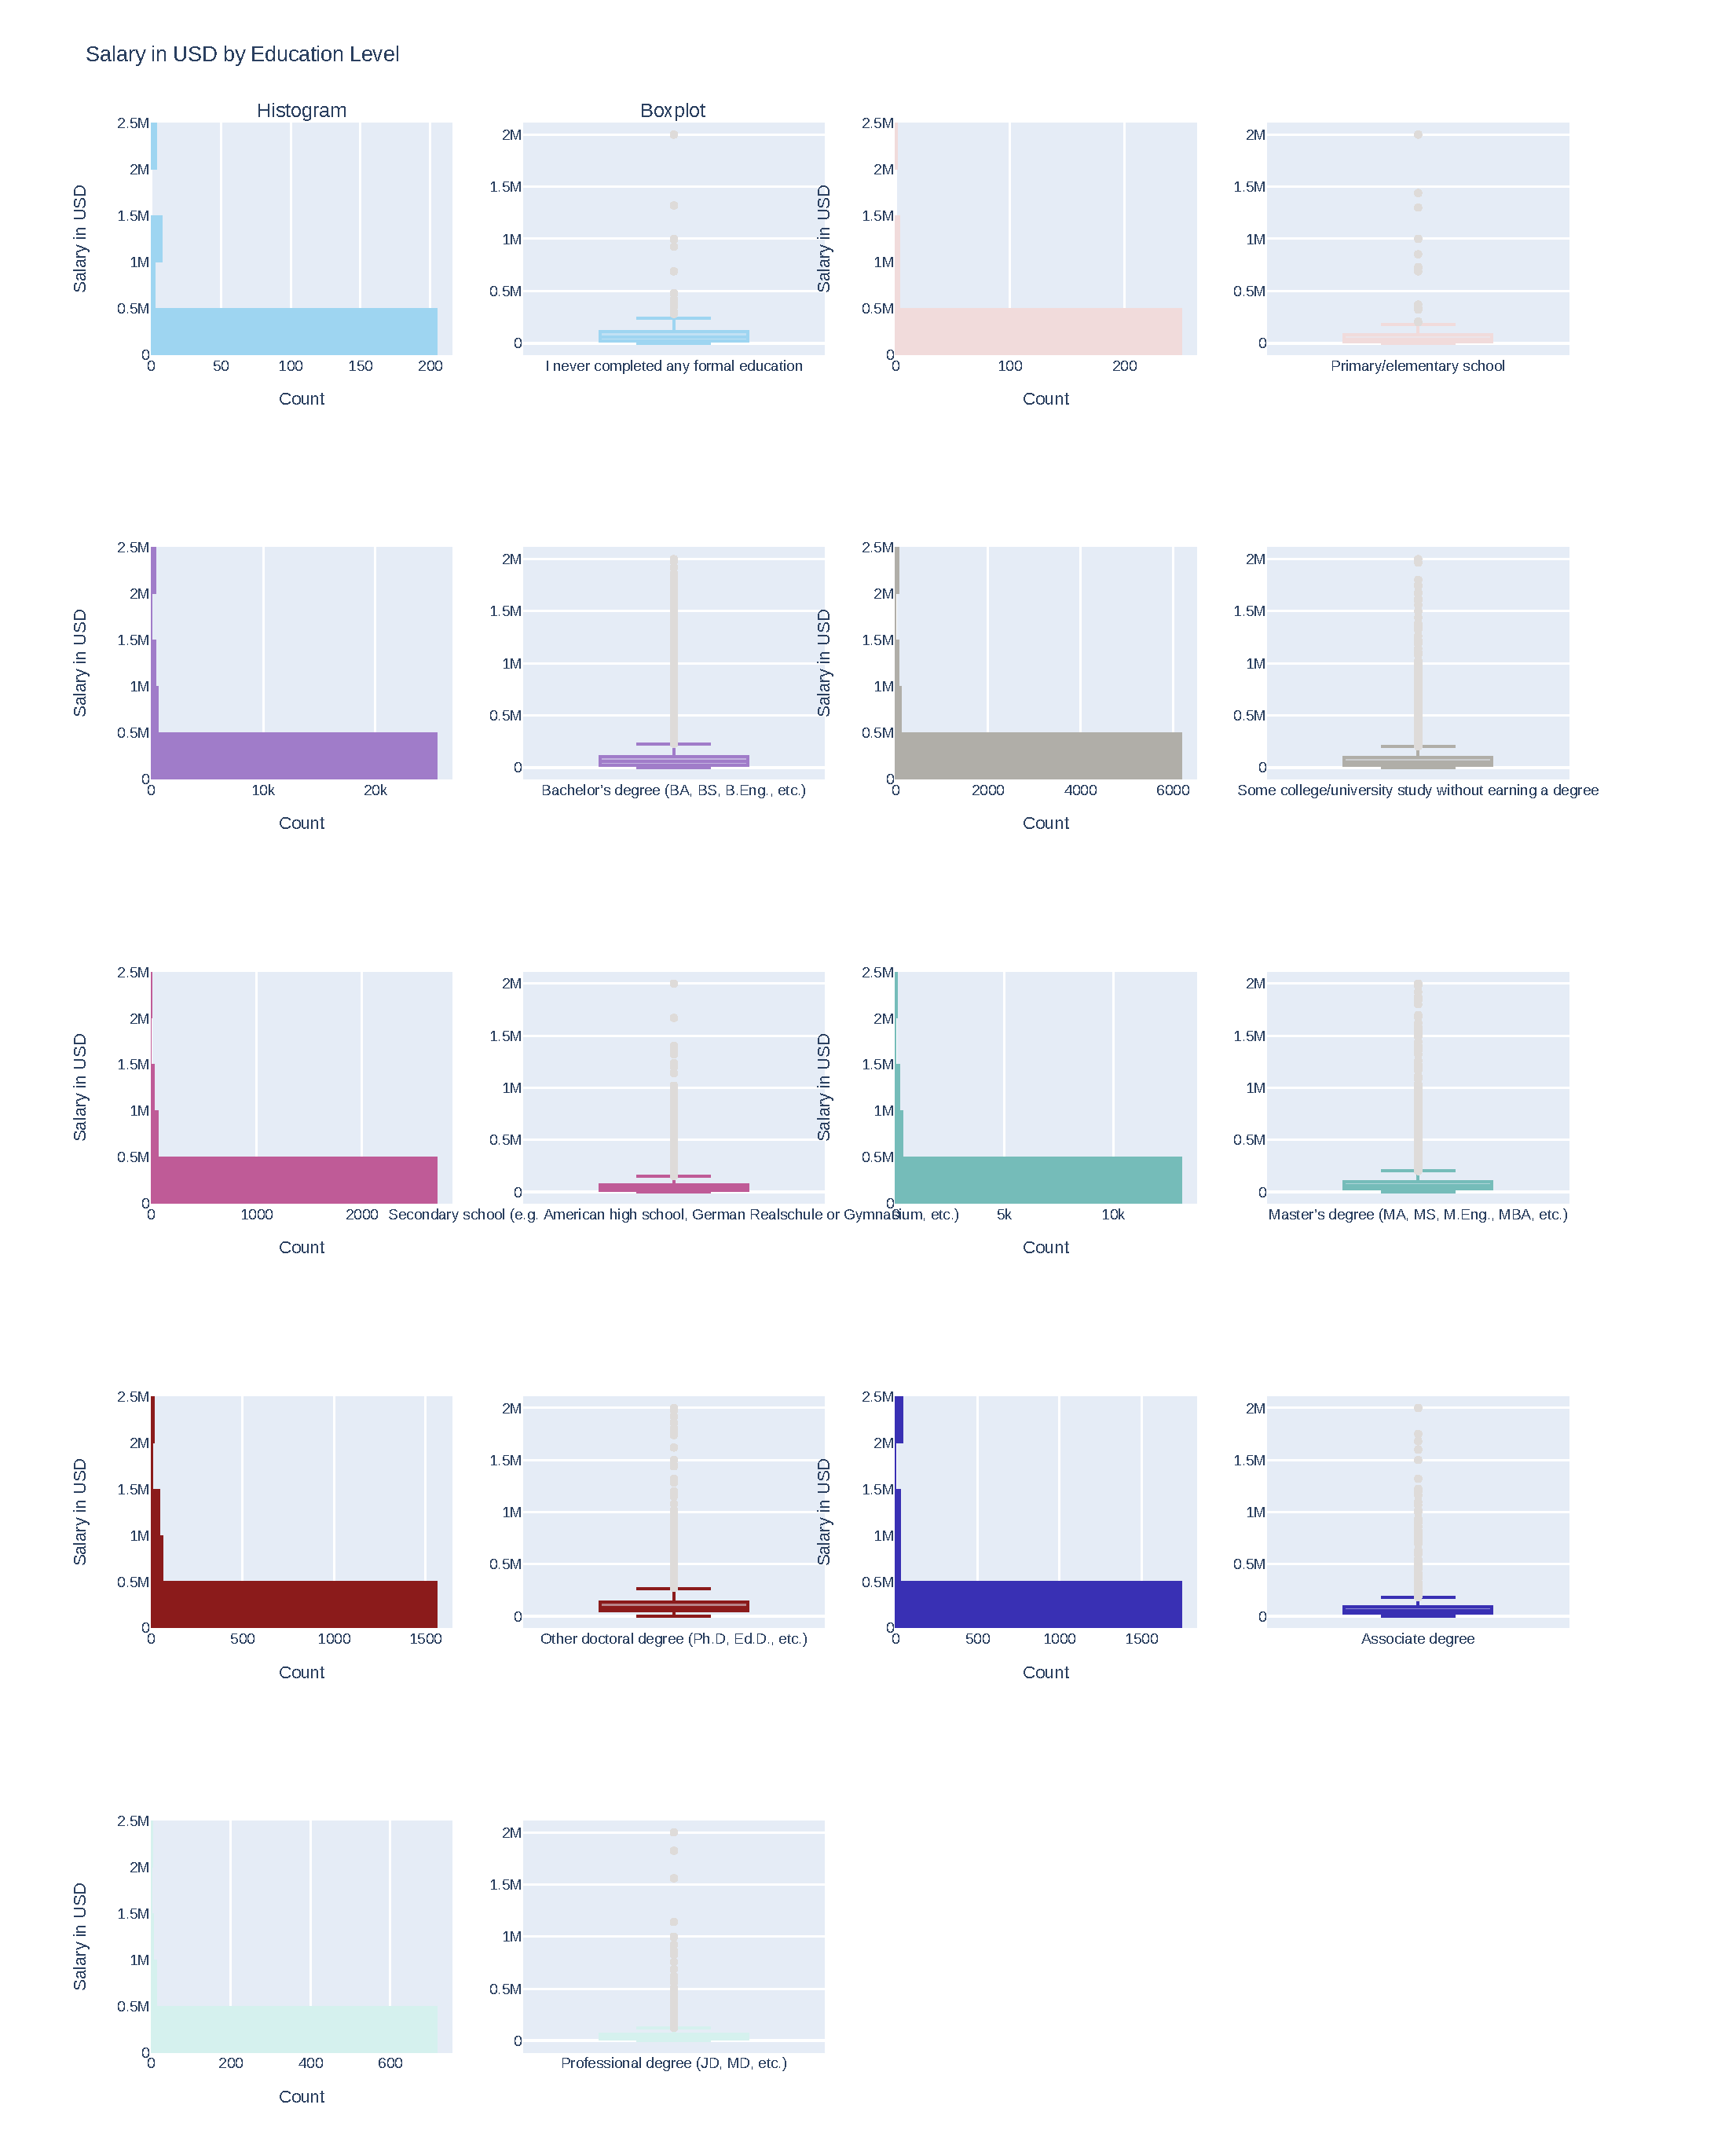
\includegraphics[width=\textwidth]{images/salary_EdLevel_hist.pdf}
    \caption{Distribution of Salary in USD by Education Level}
    \label{fig:salarybyedlevelhist}
\end{figure}

\begin{figure}[ht]
    \centering
    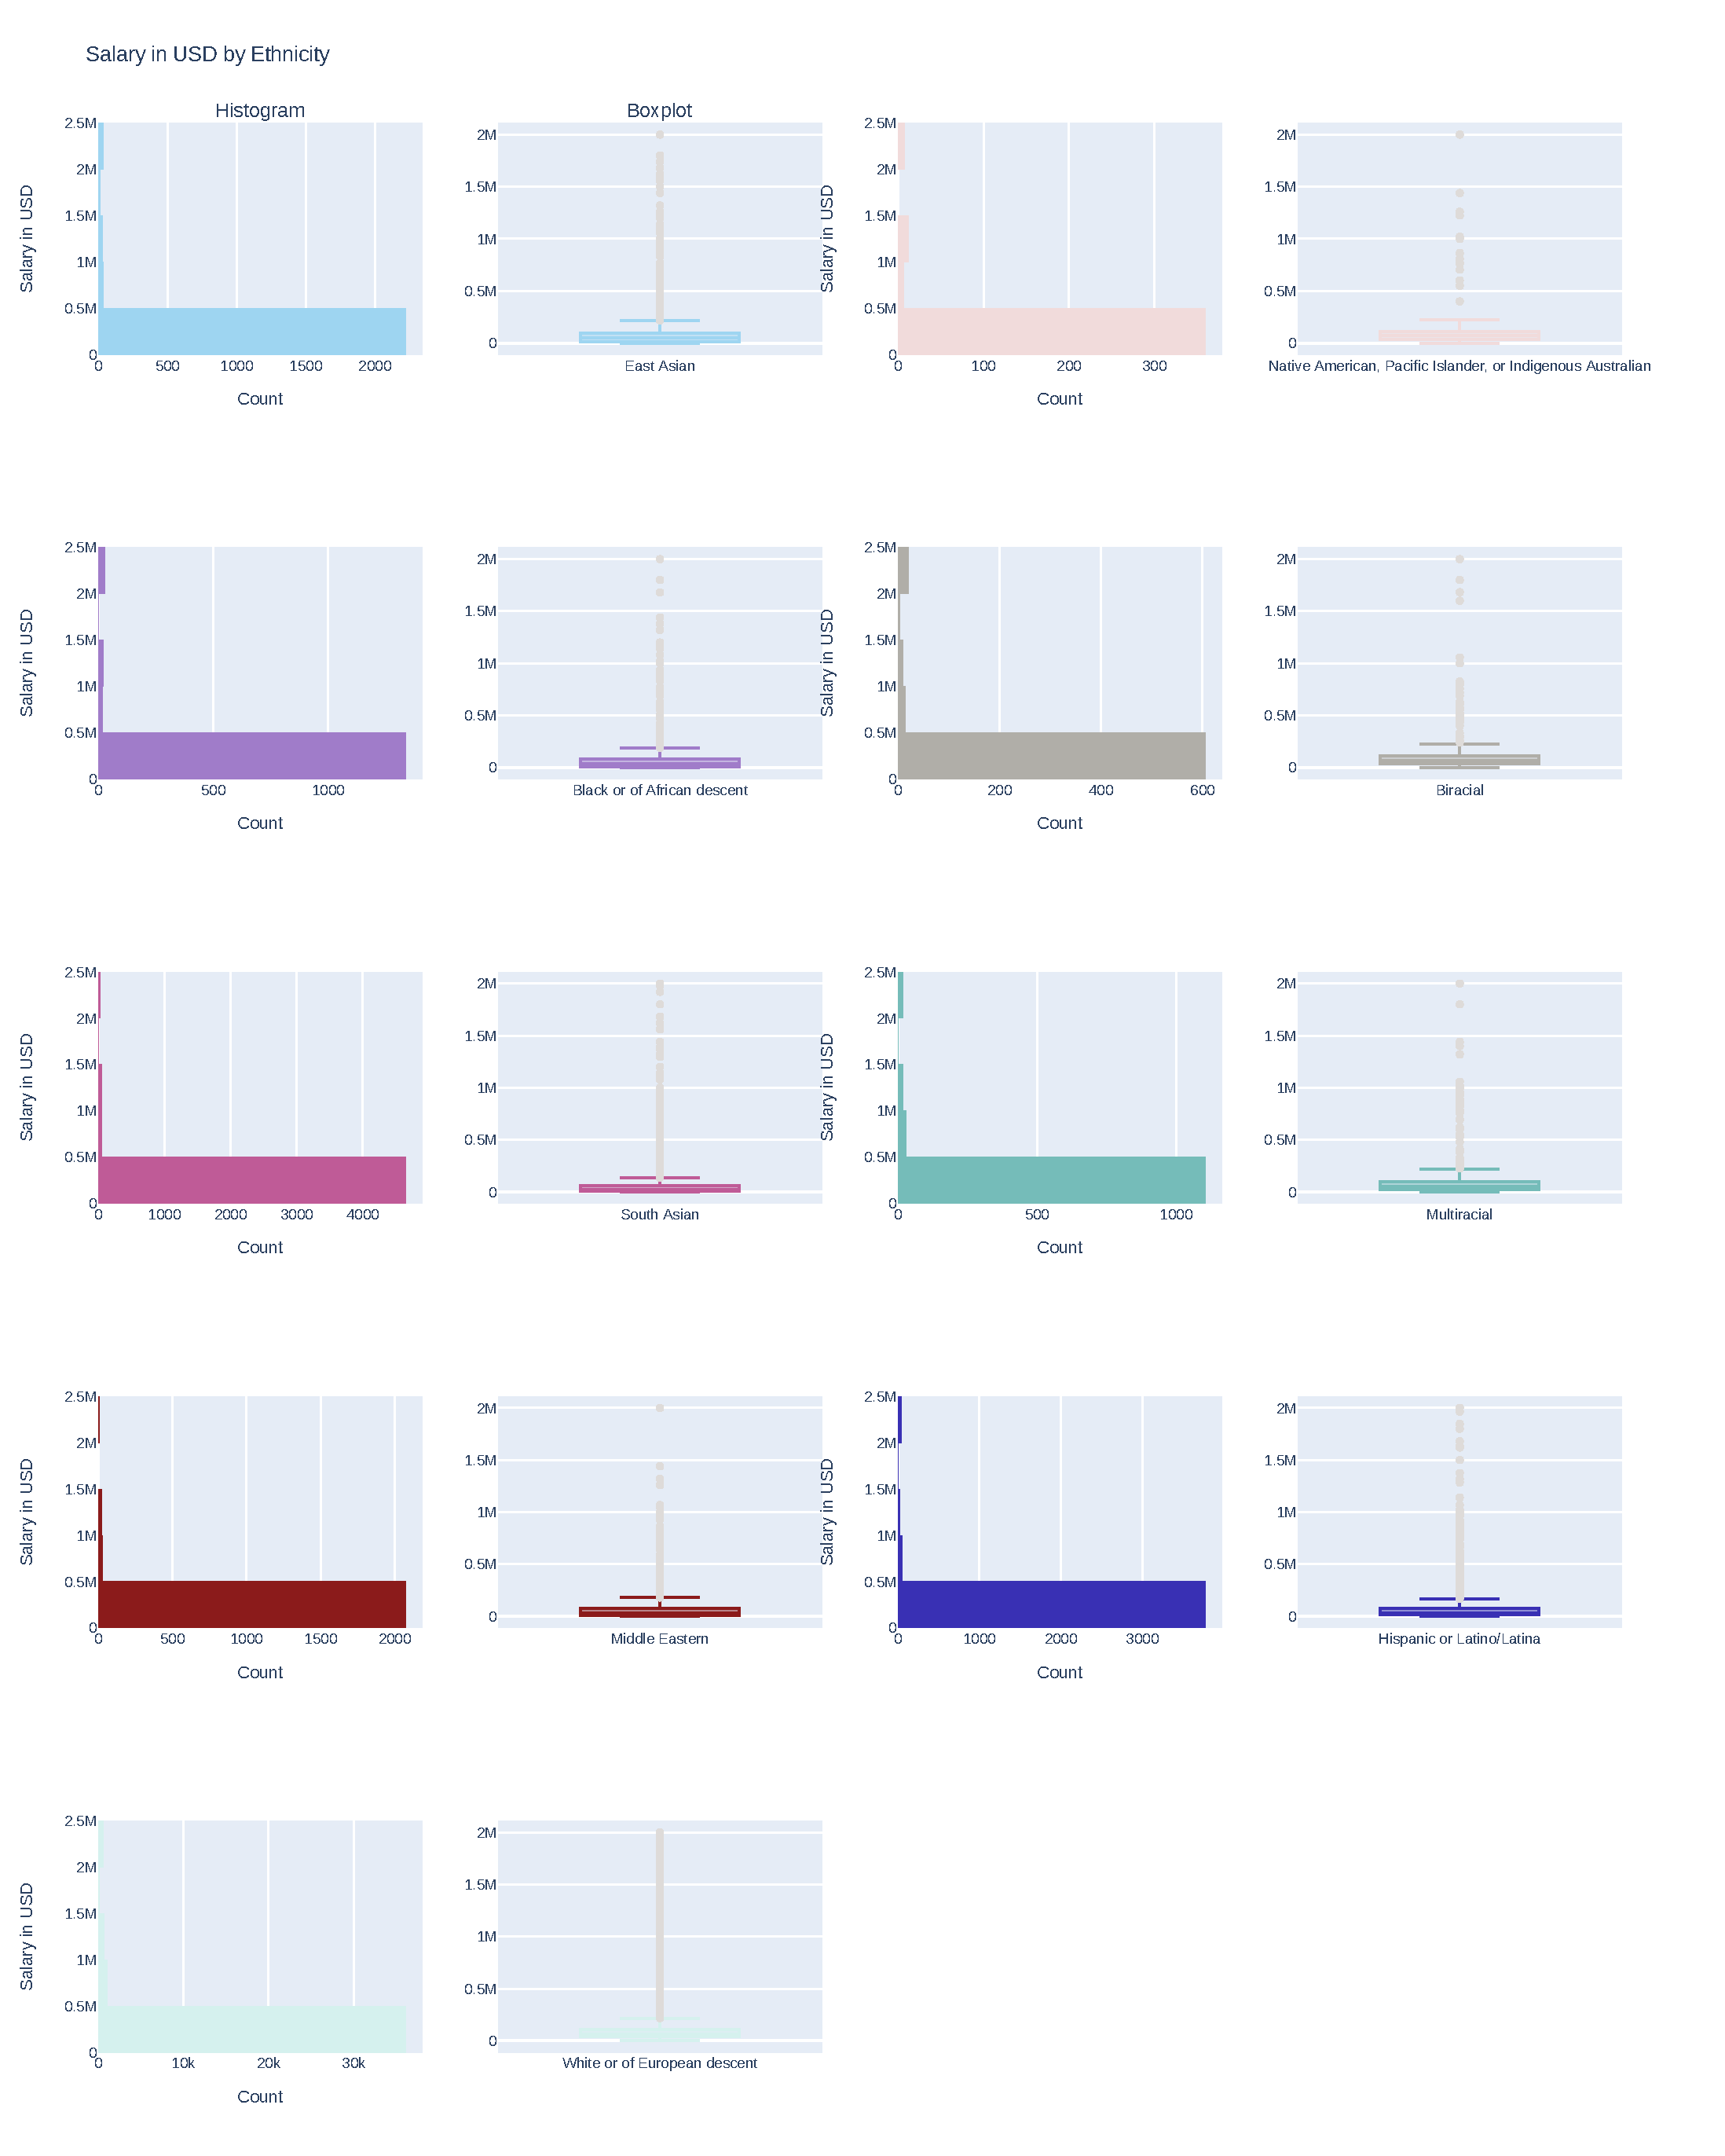
\includegraphics[width=\textwidth]{images/salary_ethnicity_hist.pdf}
    \caption{Distribution of Salary in USD by Ehnicity}
    \label{fig:salarybyethnicityhist}
\end{figure}

\begin{figure}[ht]
    \centering
    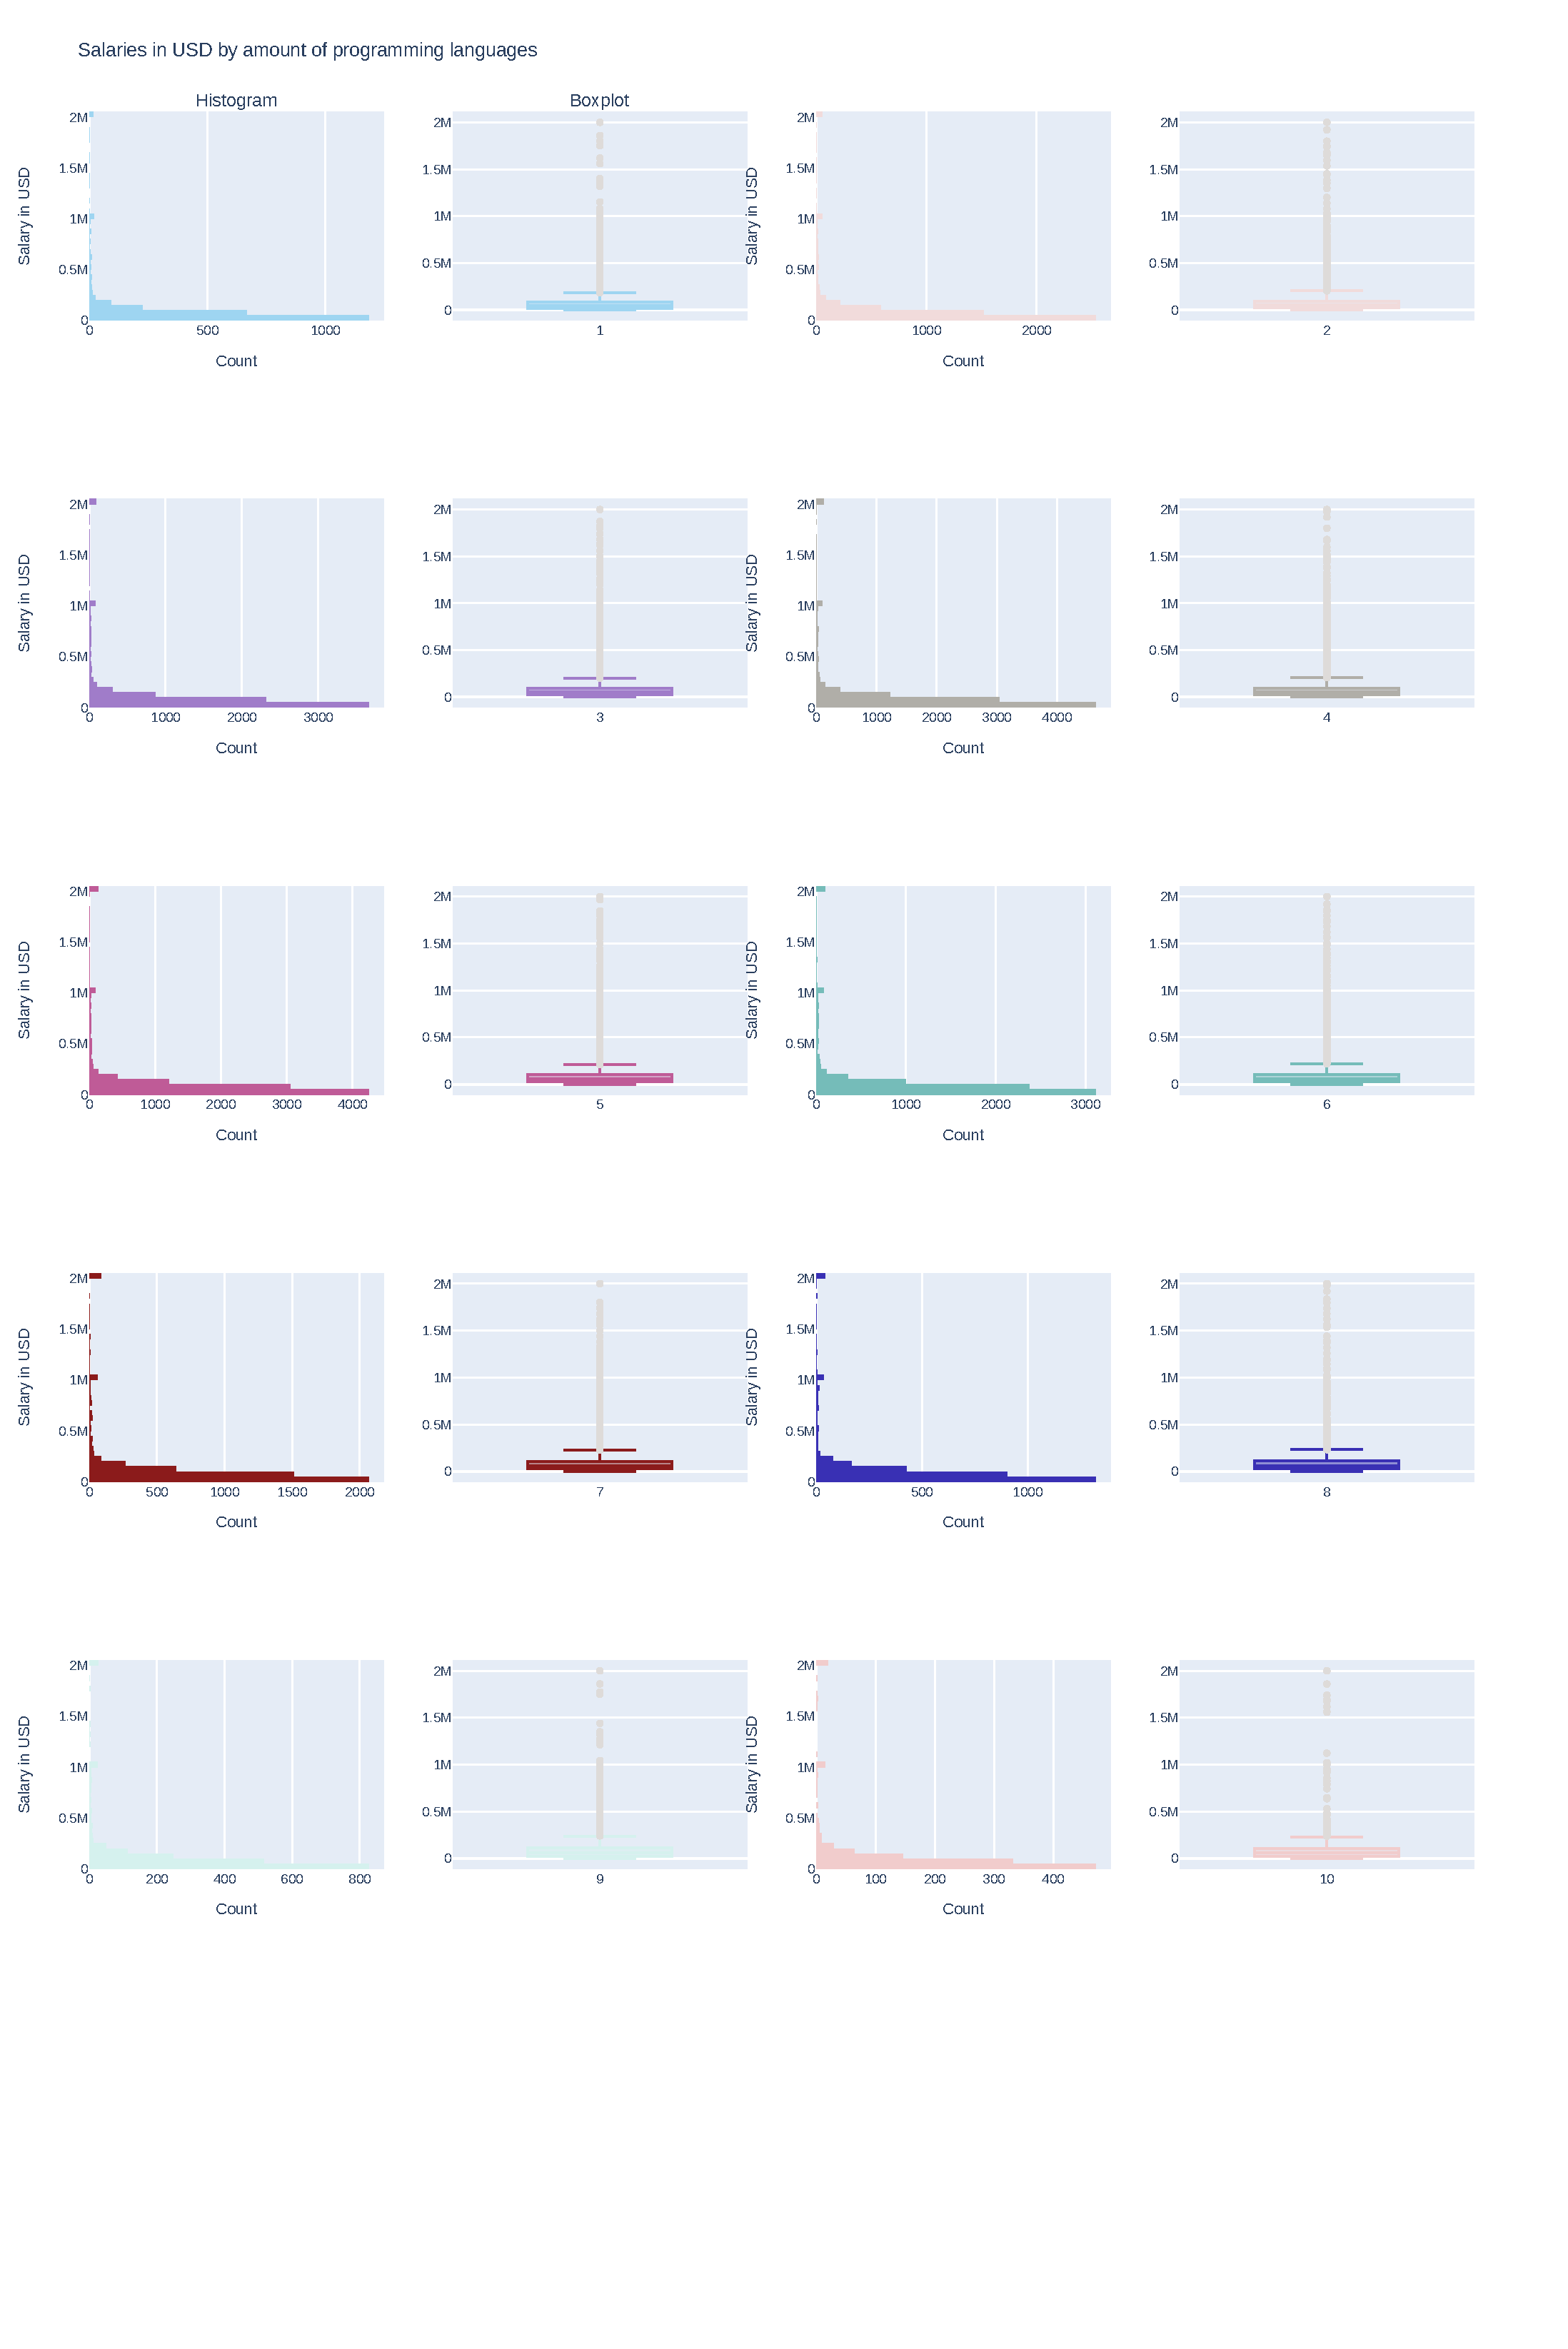
\includegraphics[width=\textwidth]{images/salary_amount_1.pdf}
    \caption{Distribution of Salary in USD by amount of languages (Part 1/3)}
    \label{fig:salarybylang1}
\end{figure}
\begin{figure}[ht]
    \centering
    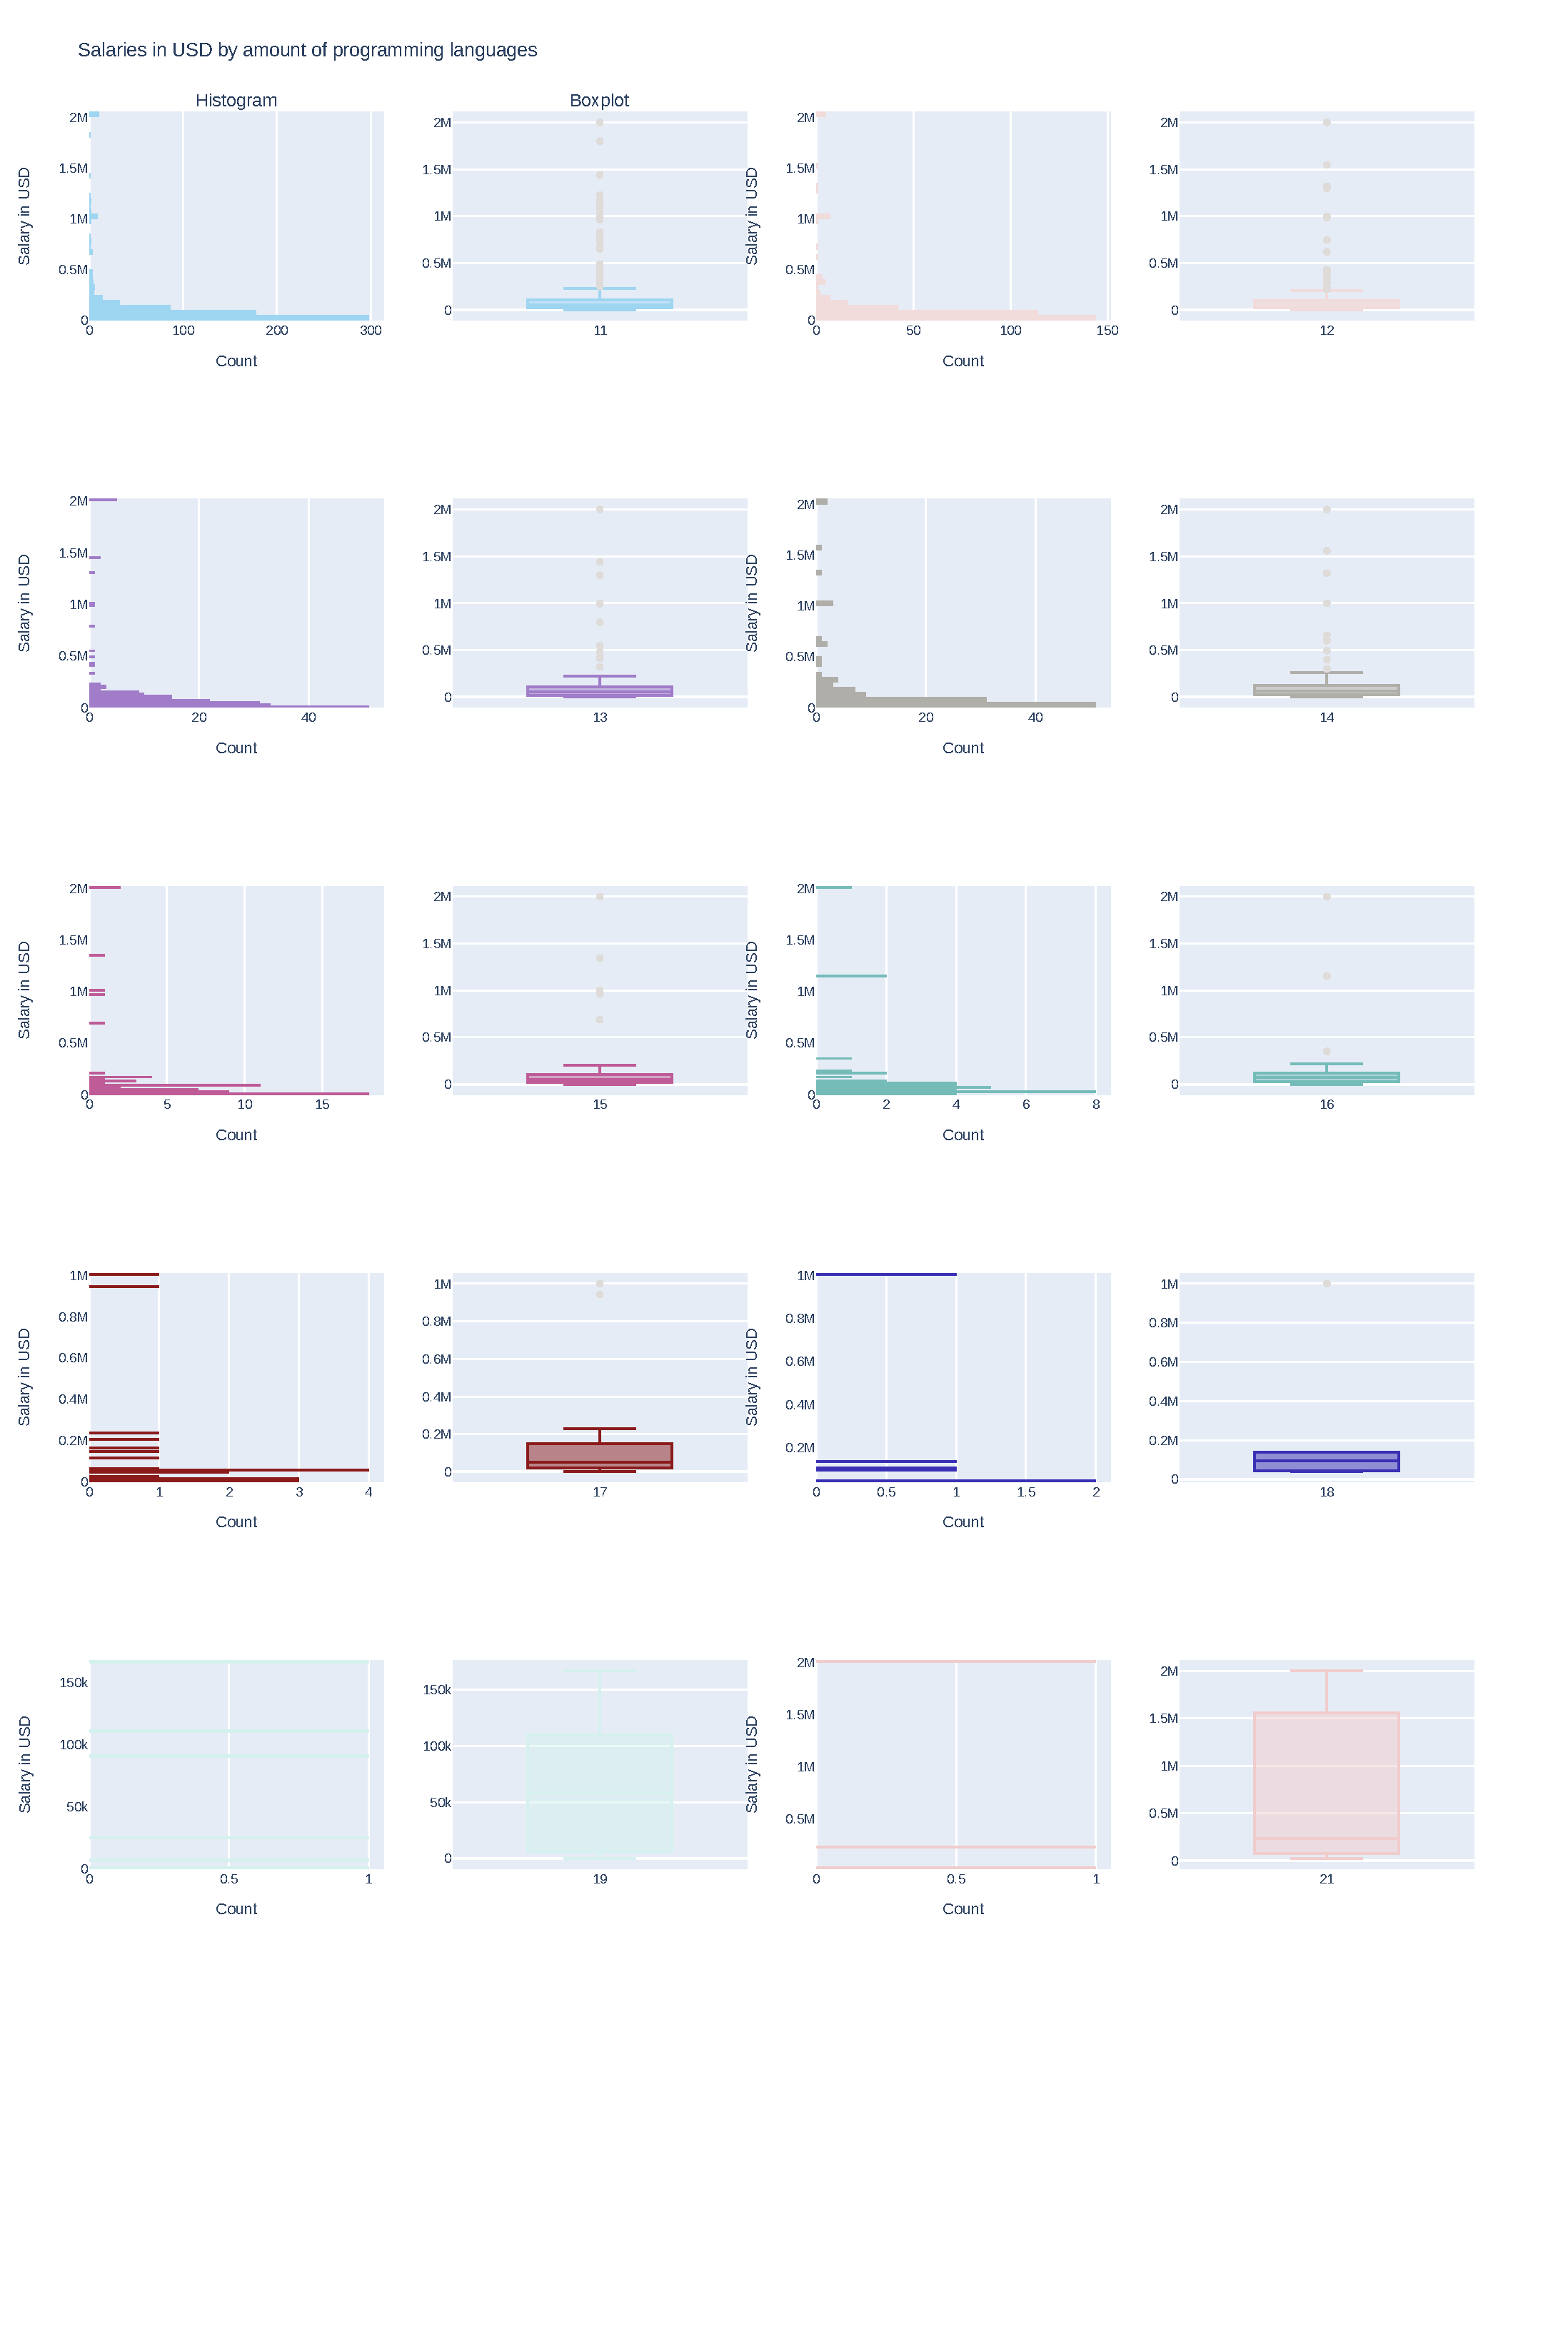
\includegraphics[width=\textwidth]{images/salary_amount_2.pdf}
    \caption{Distribution of Salary in USD by amount of languages (Part 2/3)}
    \label{fig:salarybylang2}
\end{figure}
\begin{figure}[ht]
    \centering
    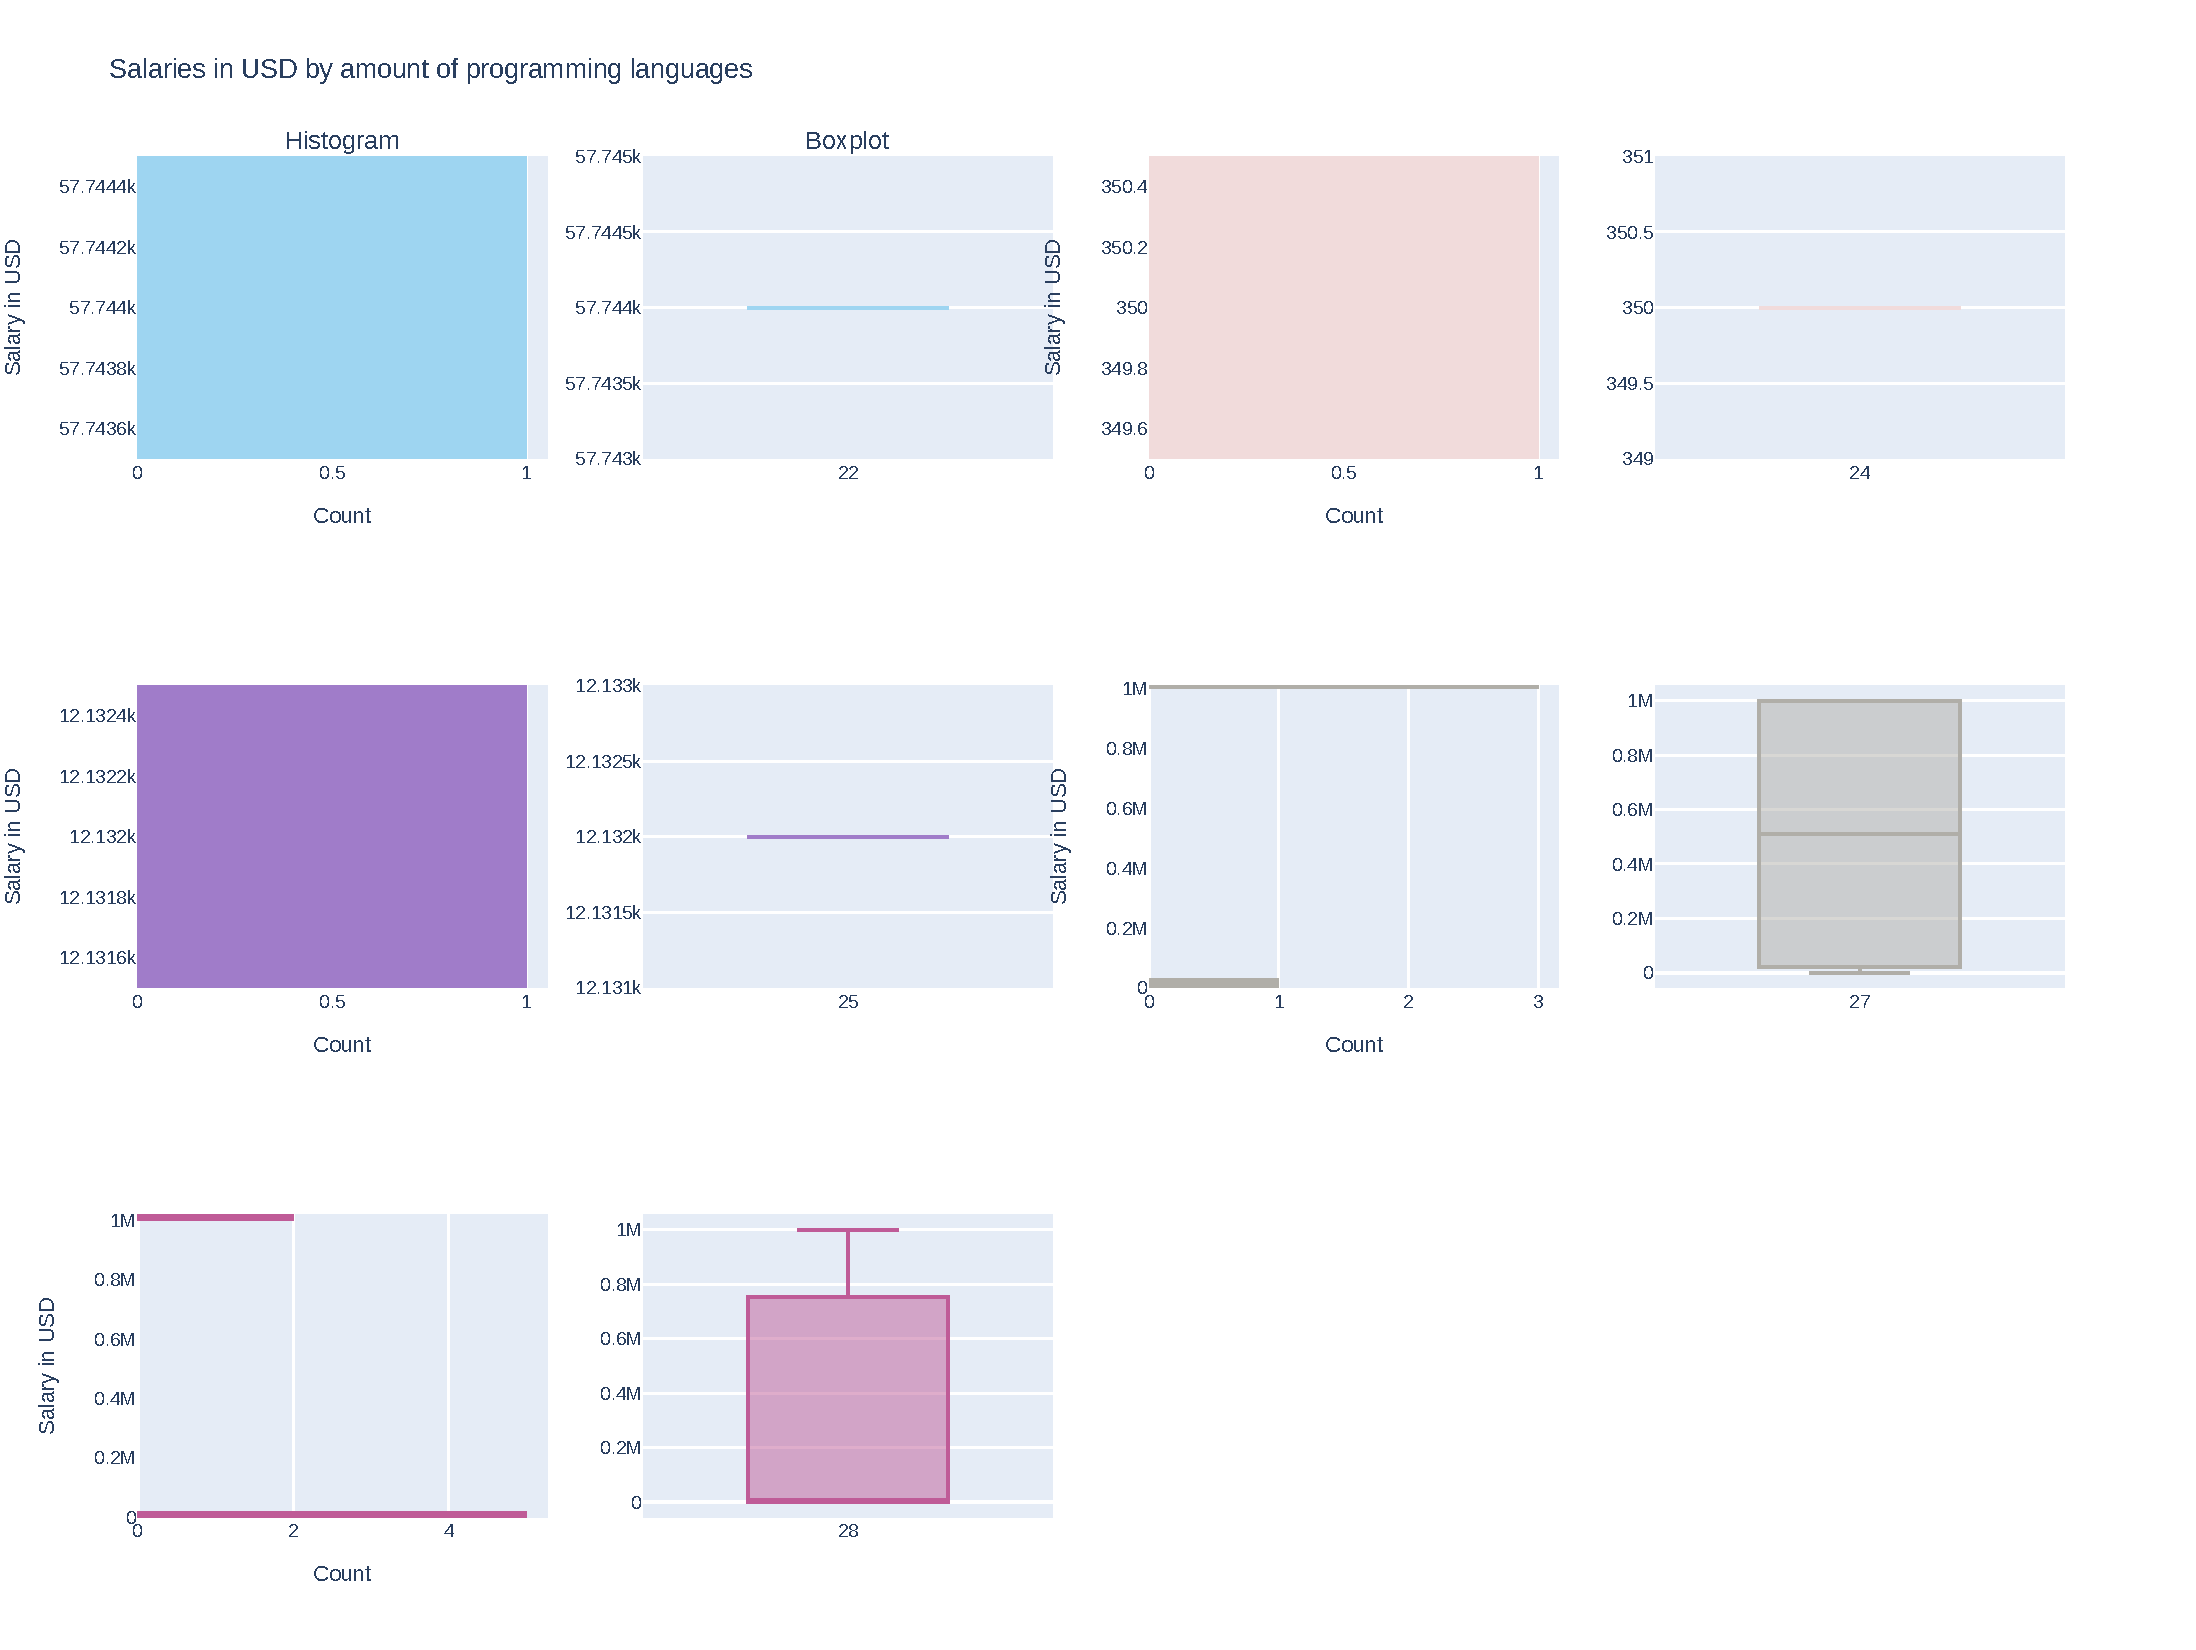
\includegraphics[width=\textwidth]{images/salary_amount_3.pdf}
    \caption{Distribution of Salary in USD by amount of languages (Part 3/3)}
    \label{fig:salarybylang3}
\end{figure}
\begin{figure}[ht]
    \centering
    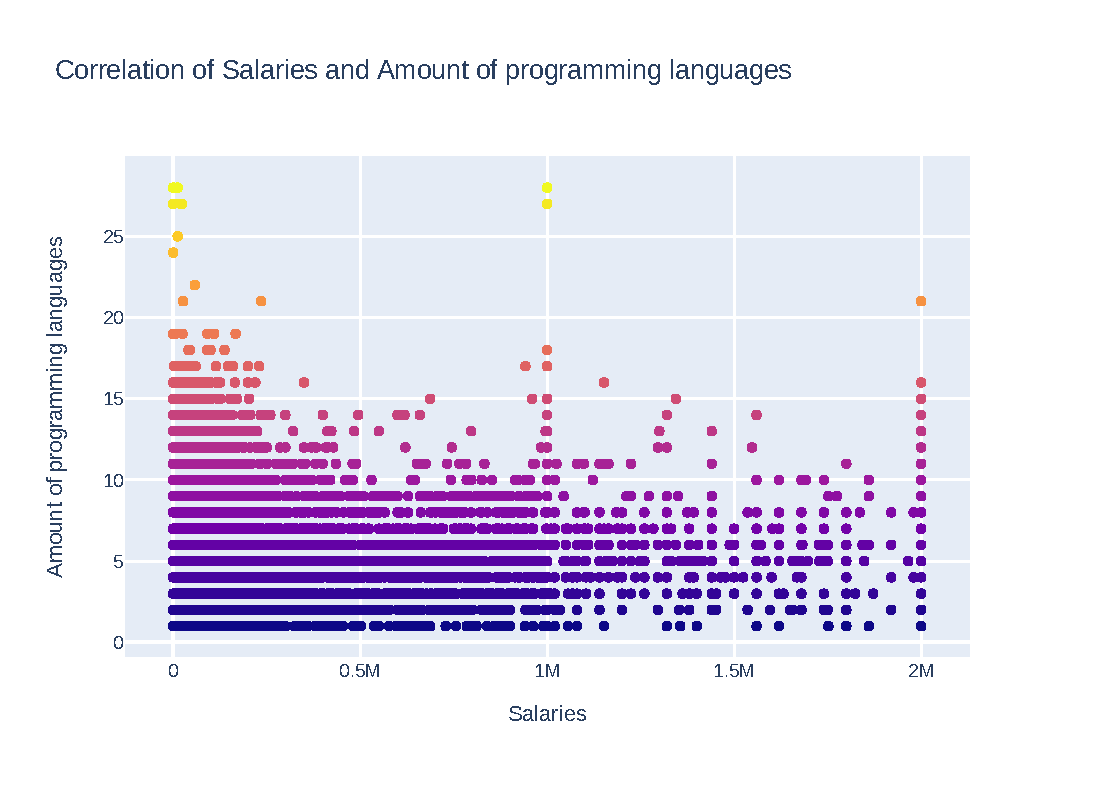
\includegraphics[width=0.8\textwidth]{images/salary_amount.pdf}
    \caption{Sactter plot of salary in USD by amount of languages }
    \label{fig:salarybylang}
\end{figure}


\clearpage
\section{Programmers}
Almost 30 different programming languages were captured by the survey where JavaScript head the list (Figure~\ref{fig:proogramminglanguages}) with almost 60K users, closely followed by HTML/CSS with 55K users. Teh five first languages are JavaScript, HTML/CSS, SQL, Python and Java. The languages with the less users are Erlang, F\#, WebAssembly,  Clojure and Elixir.
\begin{figure}[ht]
    \centering
    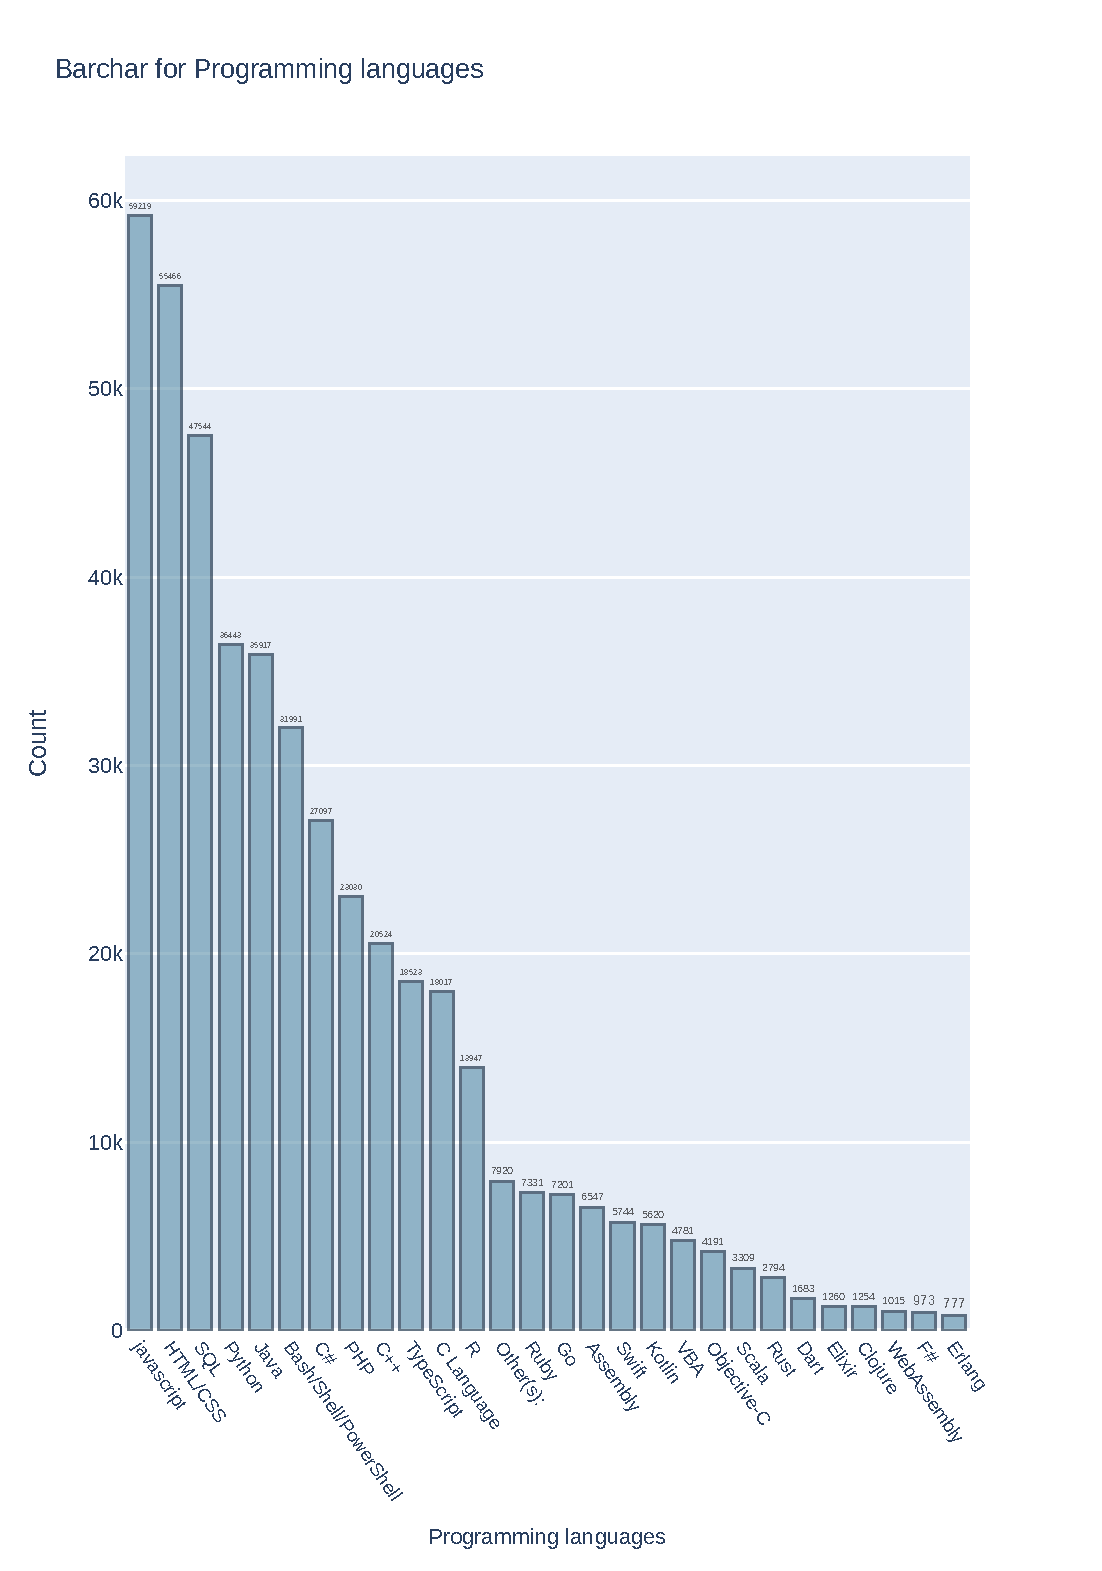
\includegraphics[width=0.8\textwidth]{images/programminglanguages.pdf}
    \caption{Used programming languages}
    \label{fig:proogramminglanguages}
\end{figure}

As an extra analyze I decided to calculate some statistical info about the salaries and the amount of user per programming language. For this calculation (Figure~\ref{fig:statisticsperamountofusers}) I decided to delimited the salaries greater than 1k and less than 2 millions to remove a little bit of outliers. The graphic shows a small relation between the salaries and the number of programmers that use certain language. For example, the five programming languages with the less number of users have better earnings that the five top ones. The interesting thing is that Golang with just 10 years of life have programmers with the best salaries above other long-lived languages like Python, Java or C.

\begin{figure}[ht]
    \centering
    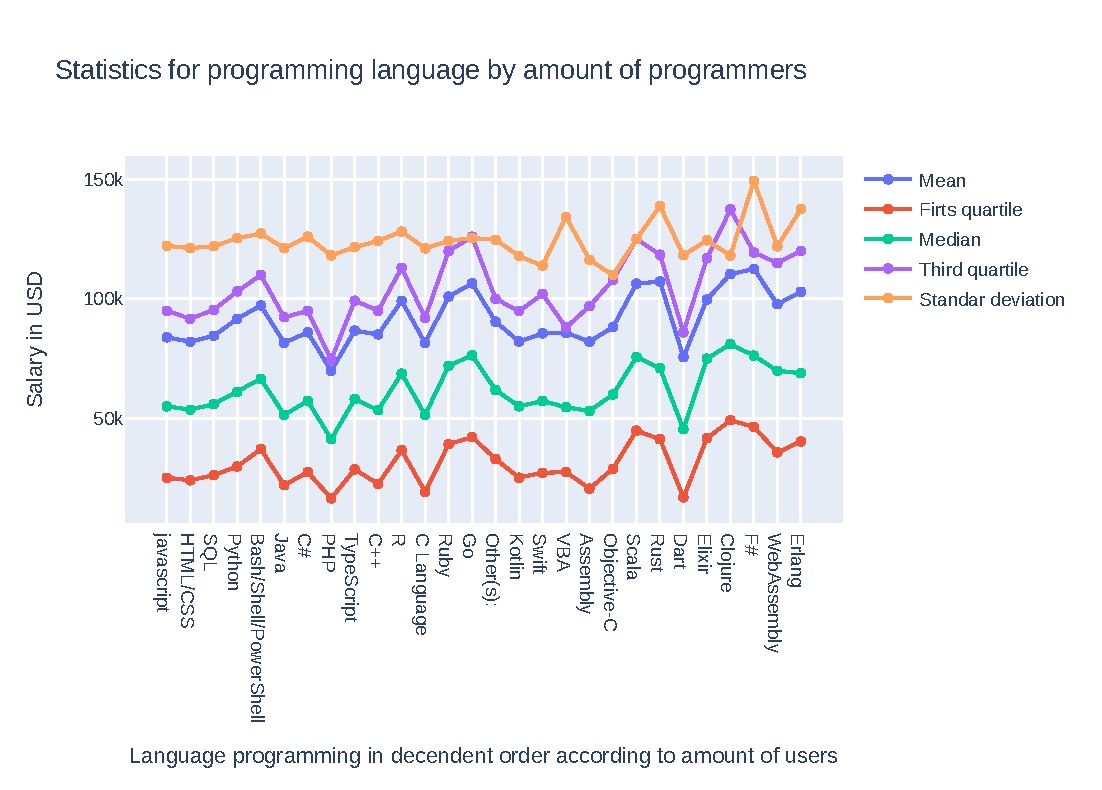
\includegraphics[width=\textwidth]{images/statistics_programm.pdf}
    \caption{Statistics per programming languages}
    \label{fig:statisticsperamountofusers}
\end{figure}{}
\section{Education}
As I mentioned before, the distribution of the salaries respect to other variables does not change, however, an expected characteristic of educations is shown in Figure~\ref{fig:salariesedlevelscatter}. This graphic shows the relation of salaries respect teh education level of the programmers and even though anybody can have a job with 2 Millions USD of salary, it is true that the programmers who have less education, their salaries are concentrated much lower than the ones with higher education.

\begin{figure}[ht]
    \centering
    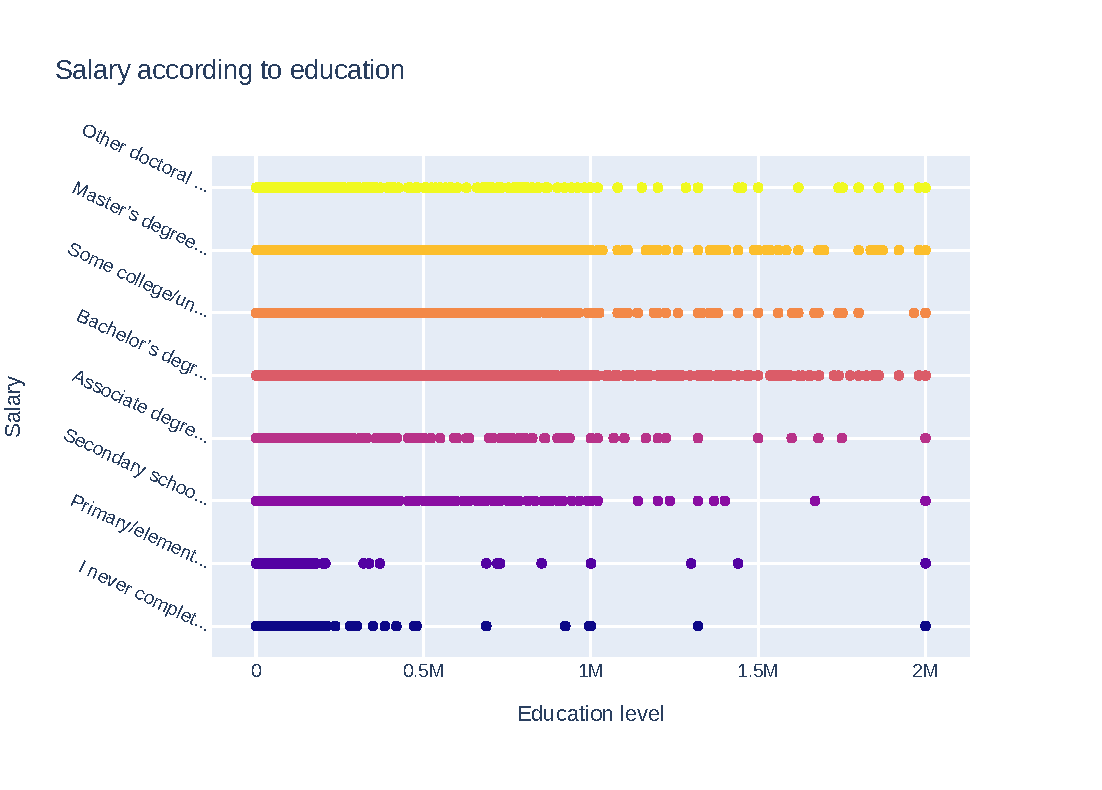
\includegraphics[width=0.9\textwidth]{images/salary_EdLevel.pdf}
    \caption{Scatter plot of Salaries respect education level}
    \label{fig:salariesedlevelscatter}
\end{figure}

Other thing about education that I have always heard it is that with a degree you will work less, so I also studied that aspect of the education and worked hours per week. Figure~\ref{fig:workedhours} shows how hours behave respect the education of the programmers. The graphic (It is delimited between 6 hours per day and 16 hour per day. With this delimitation I expected to focus the analyze in full time programmers or almost full time programmers) support the hypothesis that with higher education the spent time while programming is less than when your do not have a degree.

    \begin{figure}[ht]
        \centering
        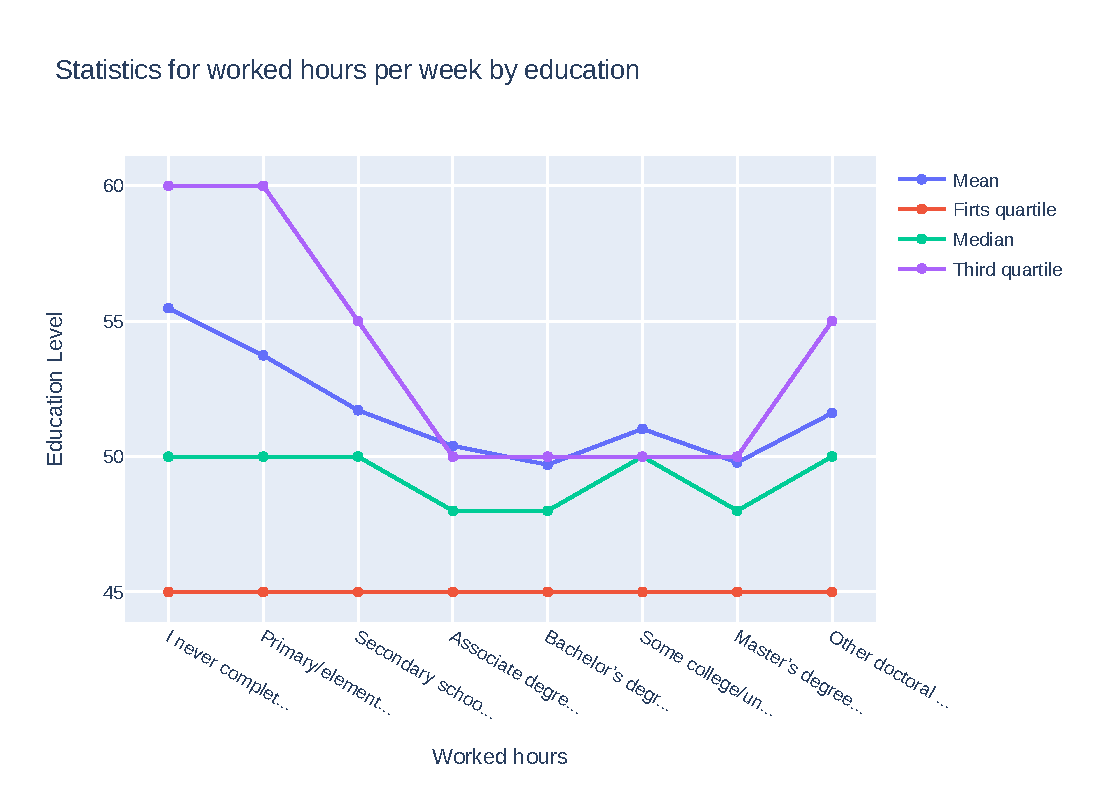
\includegraphics[height=0.4\textheight]{images/statistics_hours.pdf}
        \caption{Statistics of worked hours respect education level.}
        \label{fig:statisticshours}
    \end{figure}


    \begin{figure}[ht]
        \centering
        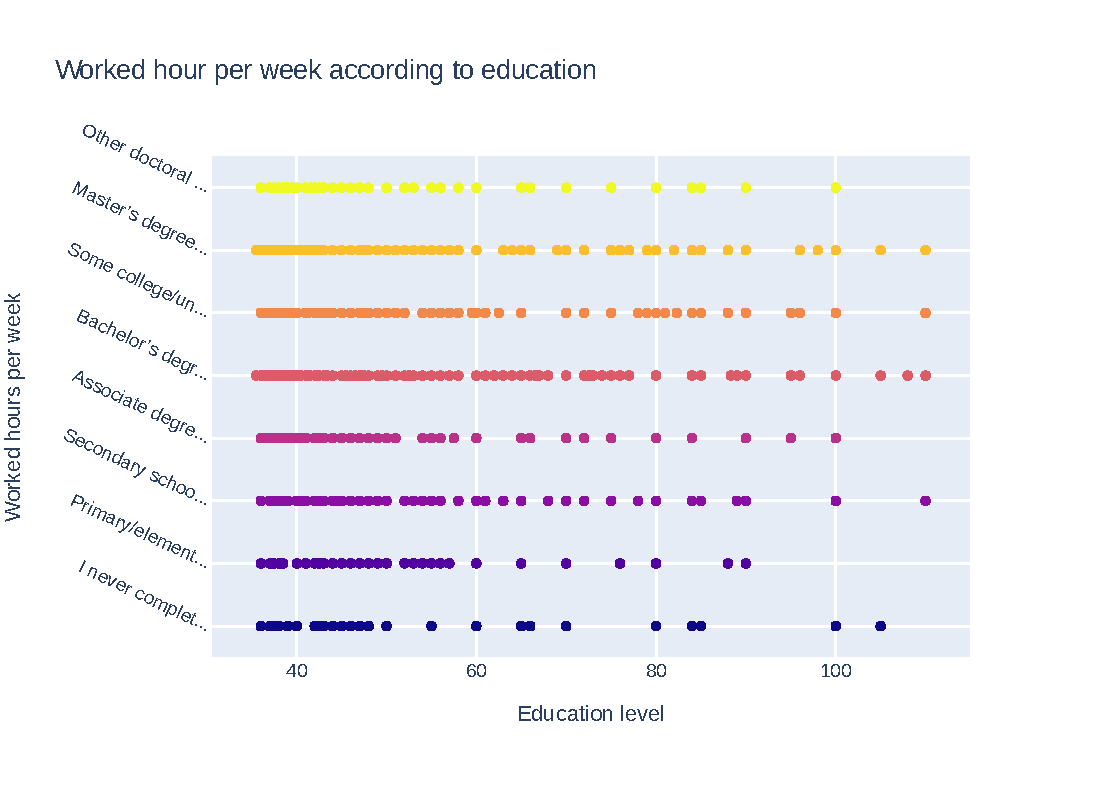
\includegraphics[height=0.4\textheight]{images/WorkedHours_EdLevel.pdf}
        \caption{Worked hours per week respect education level}
        \label{fig:workedhours}
    \end{figure}

\clearpage
\section{Gender}
The number of non-traditional gender programmers and women programmers are much much lower respect of the number of men programmers (Shown in Figure~\ref{fig:gendercount}). The interesting thing is that the non-binary gender coders have higher salaries than the men (Almost 7K USD higher as  Figure~\ref{fig:salarybygenderhist} shows). This may be due to the small sample of non-male programmers and how they are spread across all possible wages, from the lowest to the millionaires.
\begin{figure}[ht]
    \centering
    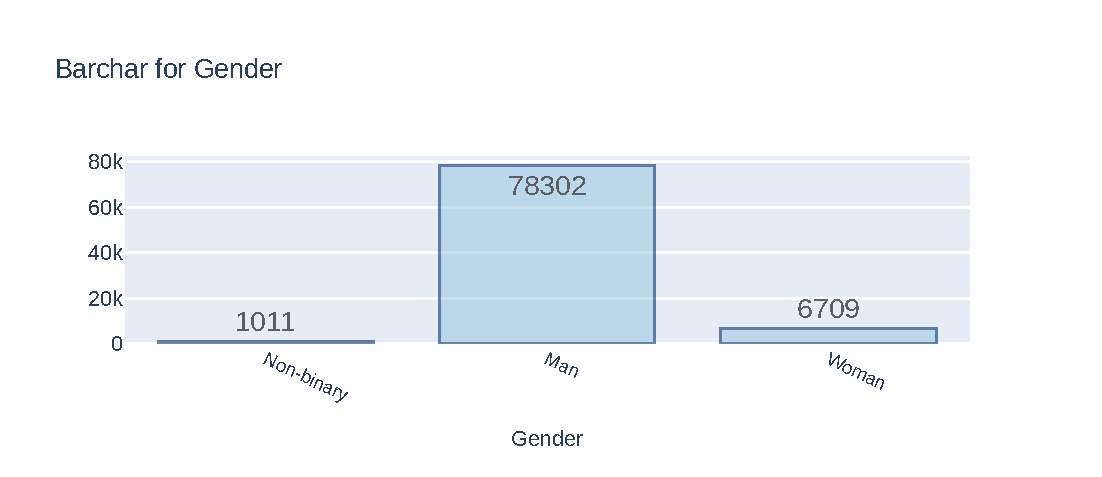
\includegraphics[width=\textwidth]{images/gender_count.pdf}
    \caption{Programmers count by gender}
    \label{fig:gendercount}
\end{figure}{}

\begin{figure}[ht]
    \centering
    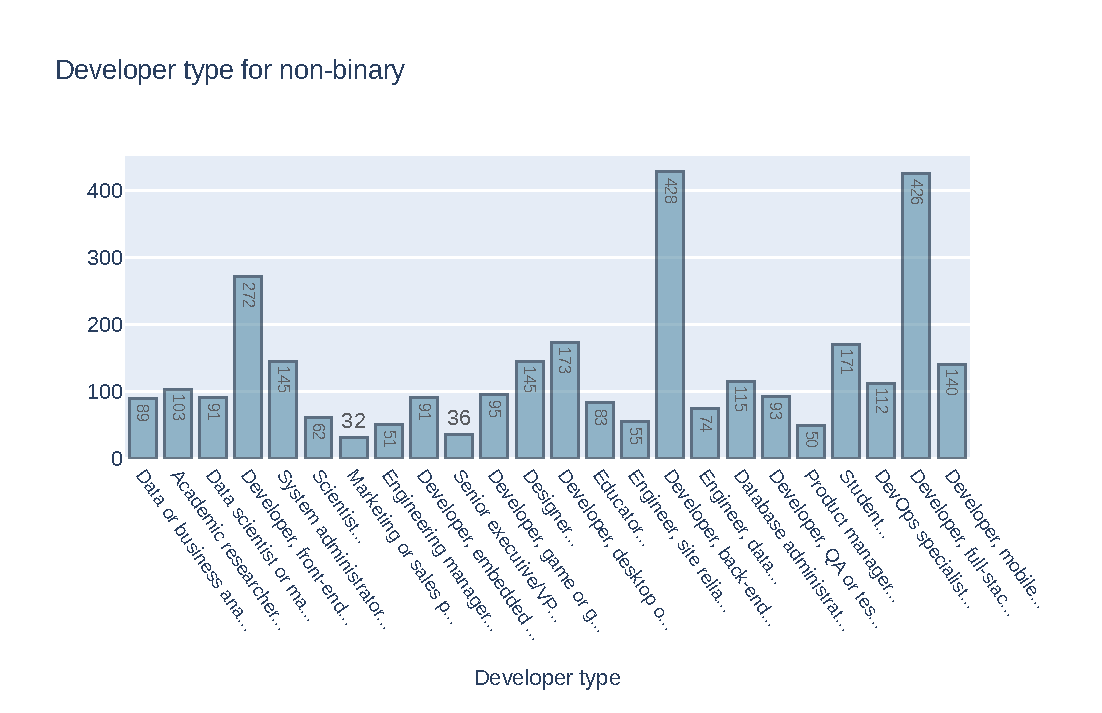
\includegraphics[width=0.9\textwidth]{images/nb_devtype.pdf}
    \caption{Developer type for non-binary}
    \label{fig:devtypenb}
\end{figure}{}
\begin{figure}[ht]
    \centering
    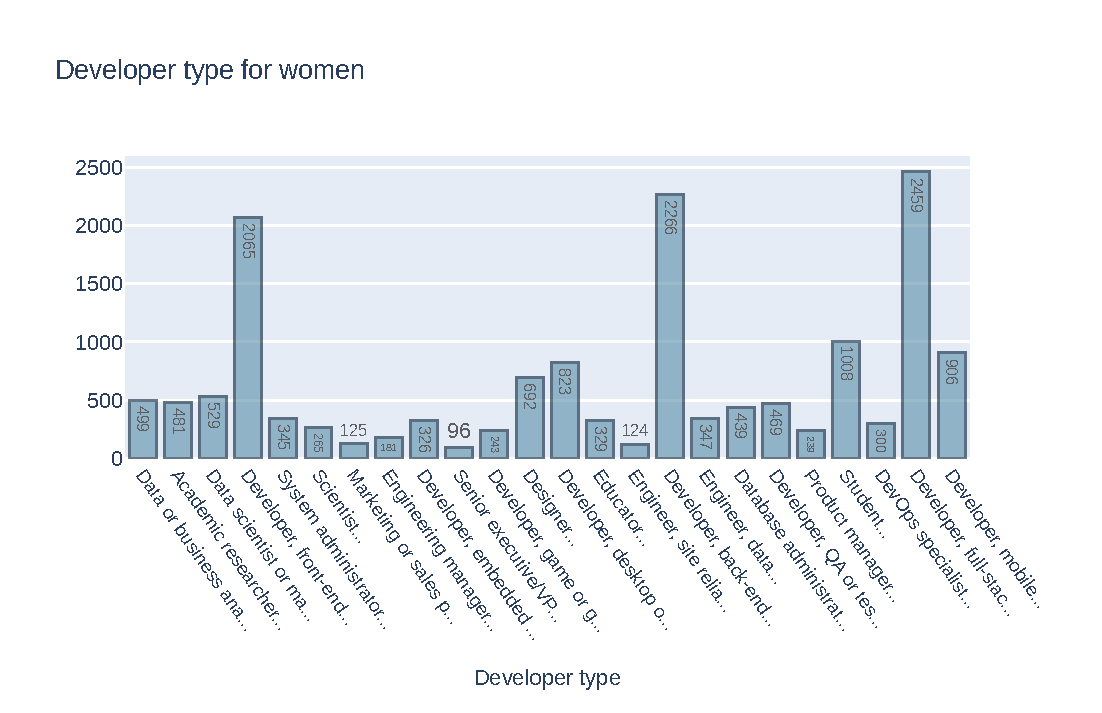
\includegraphics[width=\textwidth]{images/women_devtype.pdf}
    \caption{Developer type for women}
    \label{fig:devtypewomen}
\end{figure}{}
\begin{figure}[ht]
    \centering
    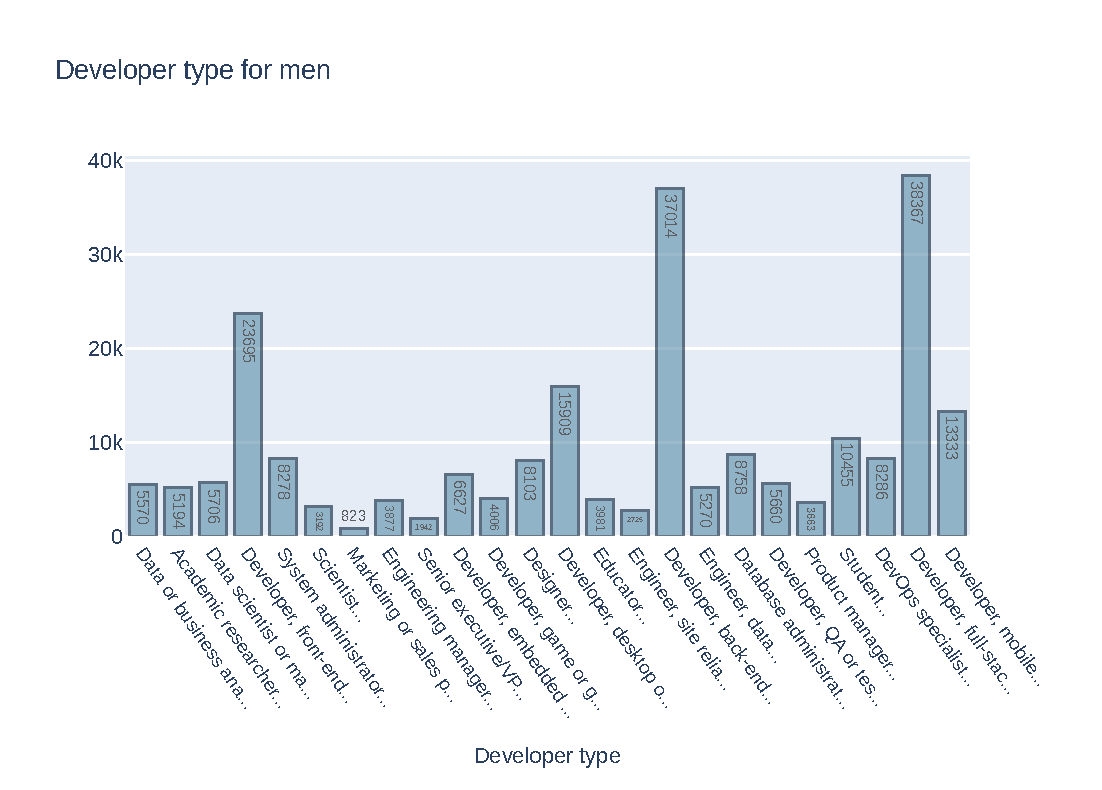
\includegraphics[width=\textwidth]{images/men_devtype.pdf}
    \caption{Developer type for men}
    \label{fig:devtypemen}
\end{figure}{}
\clearpage 
Talking about developer types, for the three genders, the web development heads the list of the most popular dev types (Fullstack, backend and frontend) and the less popular are Marketing and senior executive. The not web developers, the more abundant are desktop developer, mobile developer, system administrator and designers.
Now, the average age for men is 30 year, for women is 29 and for non binary is 28 (Figure~\ref{fig:agebygender}).
\begin{figure}[ht]
    \centering
    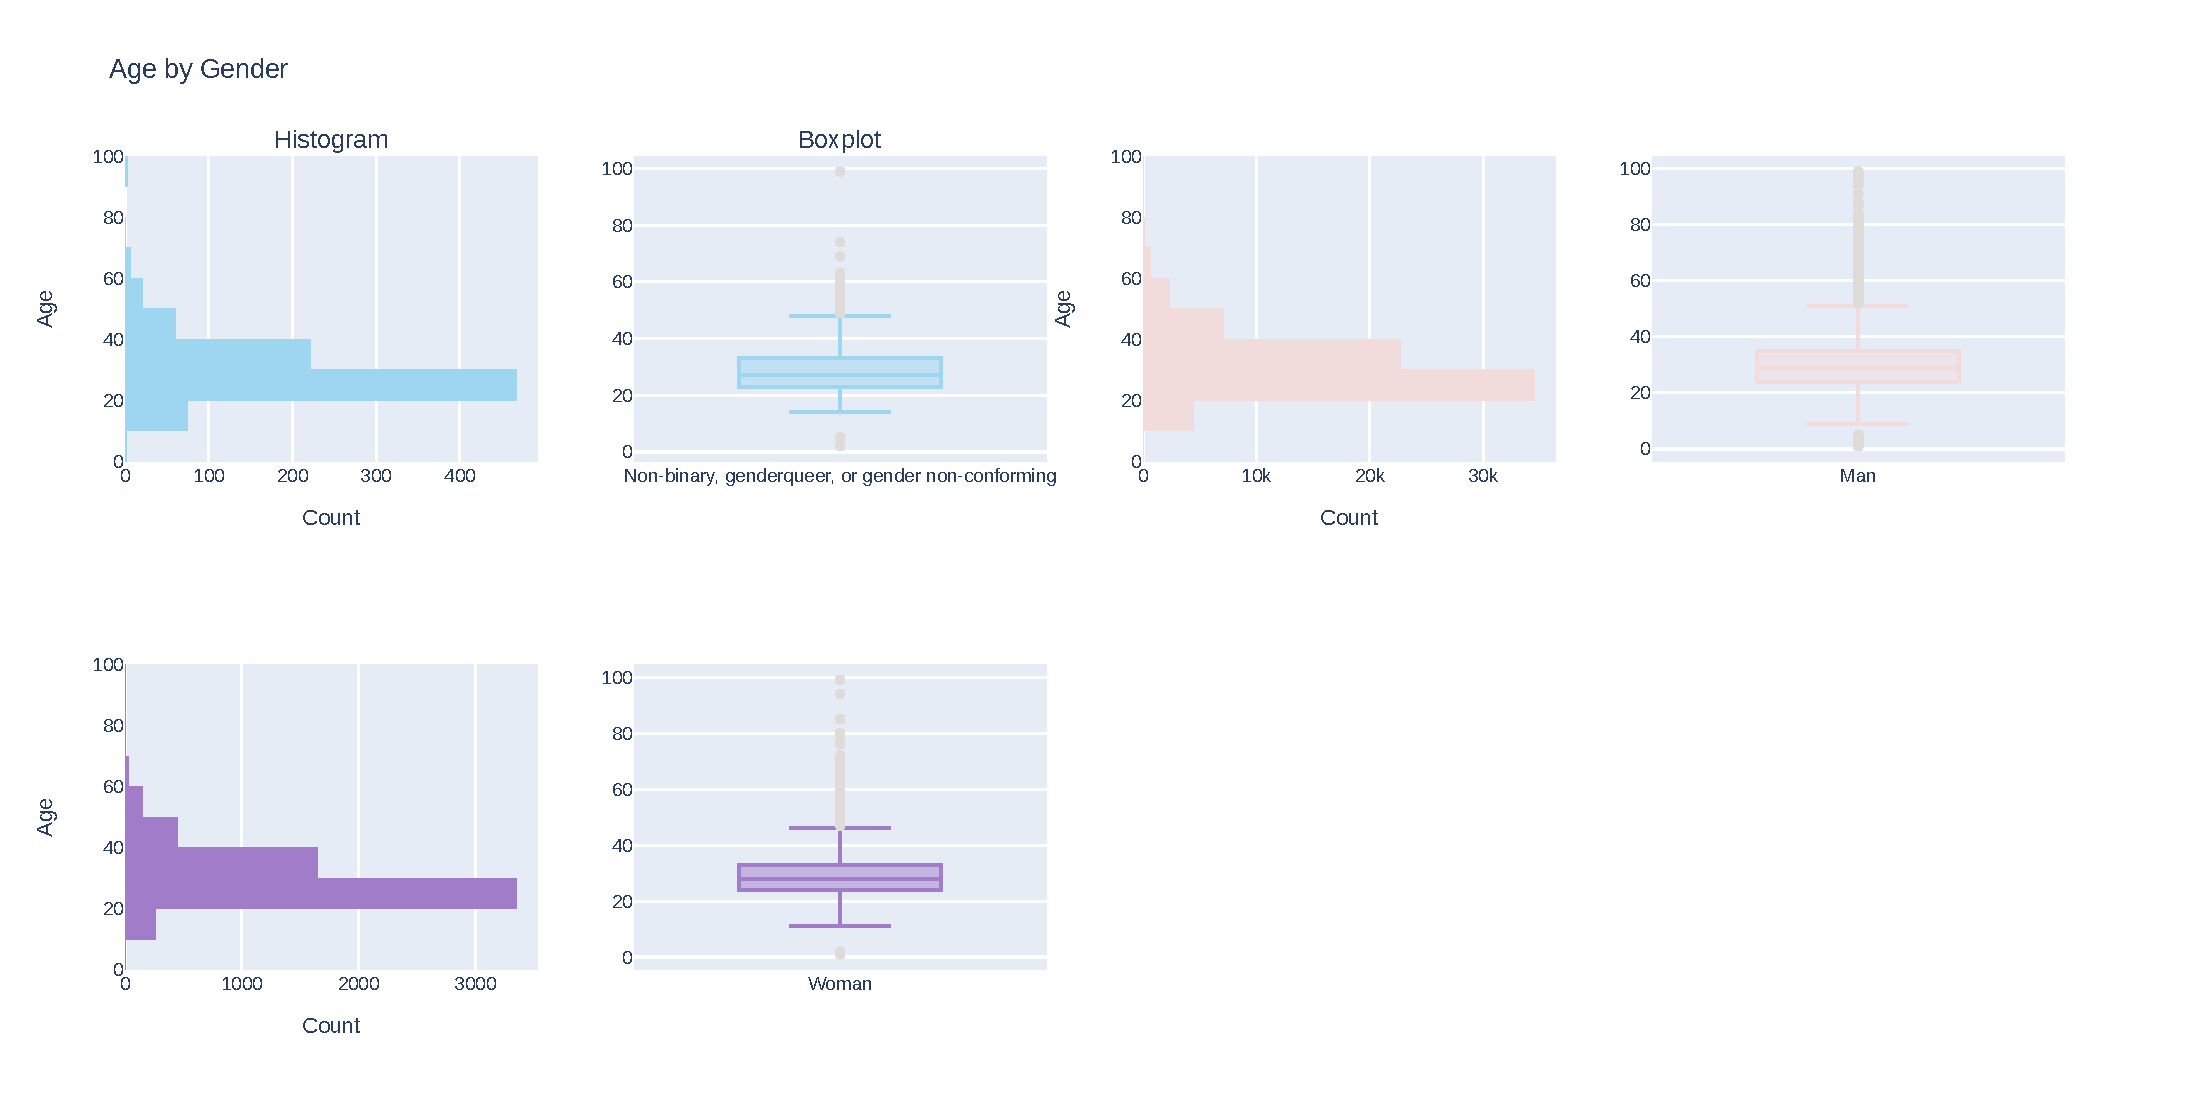
\includegraphics[width=1.1\textwidth]{images/agebygender.pdf}
    \caption{Age by gender}
    \label{fig:agebygender}
\end{figure}{}
\end{document}
